\documentclass{article}[11pt]
\usepackage[T1]{fontenc}
\usepackage{tipa}
\usepackage{titling}
\usepackage[utf8]{inputenc}
\usepackage[english]{babel}
\usepackage{hyperref}
\usepackage{csquotes}

%\usepackage{biblatex}
%\usepackage[natbibapa]{apacite}
\usepackage{natbib}
\bibliographystyle{plainnat}
%\usepackage[sort&compress]{natbib}
%\setcitestyle{numbers}
\citestyle{apa}
\usepackage{enumitem}
\usepackage{tikz}
\usetikzlibrary{trees}
\usepackage[pdf]{graphviz}
%\usepackage[pdf]{graphicx}

\setlength{\droptitle}{-6em}

%\addtolength{\oddsidemargin}{-.875in}
%\addtolength{\evensidemargin}{-.875in}
%\addtolength{\textwidth}{1.75in}
%\addtolength{\topmargin}{-.875in}
%\addtolength{\textheight}{1.75in}

\title{Syllables as a Unit for Automatic Speech Recognition}
\author{Jim O'Regan}
\date{June 2021}

\begin{document}

\maketitle

\section{Introduction}
\label{sect:intro}

The goal of this report is to design an experiment to test the hypothesis that syllables--loosely defined as vowels, or a vocalic core, in context--as a unit for the representation of speech would outperform phonemes in a speech processing task, taking into account the acoustic form, phonemic transcription, and written (orthographic) form.

The next section, section~\ref{sect:bg}, provides background to the task, concentrating on syllables (\ref{ssect:syllables}), syllabification (\ref{ssect:syllabification}), and the use of syllables in Automatic Speech Recognition (\ref{ssect:syllasr}). This is followed by a description of the experiment (section \ref{sect:experiment}), describing the corpus used (\ref{ssect:corpus}), a graphone-based approach to syllabification (\ref{ssect:graphones}), training the speech recognition systems (\ref{ssect:train}) and evaluation of those systems (\ref{ssect:eval}). Finally, there follows a discussion (section~\ref{sect:discussion}) on potential issues with the approach (\ref{ssect:issues}), and the premise (\ref{ssect:premise}).

\section{Background}
\label{sect:bg}

% I ramble on about syllables waaaaaay too long
% ...but I read so much stuff!
\subsection{Syllables}
\label{ssect:syllables}

\begin{displayquote}
\textbf{syllable} A unit of speech for which there is
no satisfactory definition. Syllables seem to
be necessary units in the mental organization and production of utterances.~\citep{ladefoged_course_2011}
\end{displayquote}

Most linguists are in agreement that the syllable is a fundamental unit of speech, but beyond that, very little is agreed. Theories about the syllable ``have been based on evidence from phonetics, phonological processes, prosody, language change, child language acquisition, and language universals.''~\citep{fallows_experimental_1981}

\begin{figure}[!h]
\caption{The components of a syllable.}
\label{fig:syll}
\centering
\begin{tikzpicture}[
  tlabel/.style={pos=0.8,right=-1pt,font=\footnotesize\color{black}},level 1/.style={sibling distance=30mm}
]
\node{Syllable}
  child{node{Onset}
    child{node{C}}
  }
  child{node{Rime}
    child{node{Nucleus}
      child{node{V}}
    }
    child{node{Coda}
      child{node{C}}
    }
  };
\end{tikzpicture}
\end{figure}

Syllables are divided into two parts: \textbf{onset} (or \textit{anlaus}), and \textbf{rime} (or \textit{rhyme}); the rime is in turn divided into the \textbf{nucleus}, which contains the vowel, or vocalic element, and the \textbf{coda} (or \textit{auslaus}). Figure~\ref{fig:syll} contains a tree diagram of the elements of a syllable. Languages vary in what a syllable may consist of, but this scheme of dividing the syllable is generally applicable to European languages.

The nucleus of a syllable usually contains a vowel; however, sonorant consonants can also function as a nucleus. In the word ``button'', ``on'' is a sonorant `n'. Czech is particularly well known for words containing sonorant `r': the tongue-twister ``Str\v{c} prst skrz krk'' \textit{(stick a finger through the throat)} contains no vowels, but all of the `r's are sonorant.

English allows syllables that follow the general template of CVC (consonant-vowel-consonant), where the onset may contain between 0 and 3 consonant sounds, and the coda may contain 0 to 5 consonant sounds, though in most dialects the maximum is 4.

\subsection{Syllabification}
\label{ssect:syllabification}

\citet{fallows_experimental_1981} lists four basic principles shared to different degrees among several hypotheses of syllabification: restrictions on segment sequences, maximal onset, stress, and ambisyllabicity.

Restrictions on segment sequences typically resolve to the idea that a sequence must be valid as the onset or coda of a word to be valid for any syllable; that syllables may only start with consonant sequences that are valid at the starts of words, and end with sequences that are valid at the ends of words. The word ``timber'' can only be syllabified as ``tim-ber'', as the sounds `m' and `b' cannot appear together in either a valid onset or coda in English words\footnote{That is, in general: there are dialects in Northern England that permit `m' and `b' in a coda; otherwise, a written `mb' is pronounced as `m'.}.

Maximal onset is a preference for the largest onset size: for example, the word ``happy'' could be syllabified as ``ha-ppy'' or ``happ-y'': maximal onset would select ``ha-ppy''. Technological approaches to syllabification tend towards maximal onset~\citep{ladefoged_course_2011}, and this is the default for many languages (for example, Hawaiian syllables have no coda, while Japanese and Chinese restrict codas to nasals).

Stress is typically considered in connection with maximal onset: the stressed syllable is first segmented to have maximal onset, unstressed syllables are treated after, in various ways. \citet{wells_syllabification_2019} argues 
%unconvincingly
that stressed syllables should have maximal coda in addition to maximal onset.

Ambisyllabicity is, in its strictest sense, the idea that a consonant between two vowels can belong to both; other interpretations can allow for variation in syllabification, or sharing of certain sounds only. Gemination, or consonant lengthening, is often realised as a repetition of the consonant. Doubled consonants in English do not automatically signify gemination, as they do in Italian or Swedish, but they do in compound words (``midday'') or prefixed words (``misspell''); in these cases, the lengthened consonant is typically considered to be split in half, with the halves acting as the end and beginning of two syllables.
%Gemination? Polish, Italian & Swedish have a slightly different form of ambisyllabicity where two 'halves' of a long/geminated consonant are split between syllables.

\citet{goslin_comparing_2007} sort syllabification methods into two broad categories: ``legality'' (restrictions on segment sequences, as above), and sonority.

Sonority methods use a ranking of sonority, or loudness, of phonemes, so that sonority maximally rises towards the vowel, and maximally lowers away from it: in ``dormant'', the liquid `r' is ranked higher in sonority than the nasal `m', so ``dor-mant'' is the best syllabification.

This is according to the hierarchy given by \citet{kingston_role_1990}: vowels $>$ glides $>$ liquids $>$ nasals $>$ obstruents\footnote{For brevity, by example of the letters most associated with these sounds in English: \textit{glides} (semi-vowels): y, w; \textit{liquids}: r, l; \textit{nasals}: m, n, ng; \textit{obstruents}: f/v, s/z, t/d, p/b, sh/`zh', ch/j, k/g, paired as voiceless/voiced (with/without using the vocal cords).}, though there are several other hierarchies: \citet{katamba_introduction_1989}, for example, has: vowels $>$ glides $>$ nasals $>$ voiced obstruents $>$ voiceless obstruents; \citet{ladefoged_course_2011} give a hierarchy for individual sounds, estimated from acoustic data, but only for a few of the sounds of English.

\citet{saussure_course_1959} mentions sonorant fricatives as a criticism of sonoric syllabification; for English, at least, these hold equally for legality-based syllabification: in English, in general, words cannot start with `bz', `ps', or `pf', yet we have interjections `bzz', `psst', `pff'.
%although in fast speech the realisation can be one of these,
% nah, I've written too much already

% I was going to also look for how the existance of mono-syllabic words influences syllabification - Wells' maximal coda has ``dolphin'' segmented as ``dolph-in'', which matched the intuition of zero people I asked; my son specifically mentioned the existance of ``doll'' and ``fin'' as influencing his syllabification; the example below was intended to show that even taking words into consideration, syllabification can still be ambiguous.
% I'm scribbling this to keep myself writing, don't mind me.
%``particular'' could be broken into words as ``par tic you Lar'' or ``part ick yule are''.

\subsection{Syllables in Automatic Speech Recognition (ASR)}
\label{ssect:syllasr}

Phoneme-based systems have been dominant in ASR for some time, in large part because they are ``inherently free from vocabulary limitations''~\citep{lopes_phoneme_2011}--that is, new vocabulary can be added to such a system at any time by adding its transcription to the lexicon, or by enlarging its language model\footnote{The language model gives the probabilities of words in sequence, which is useful in the case of phonetic ambiguity: ``made a mistake'' is far more likely than ``made a miss take'', and so on.}; they are not inherently tied to the use of phonemes, however.

Syllable-based systems can be found in the earliest days of ASR: \citet{fujimura_syllable_1975} is situated in a context of ASR systems that used template-matching to recognised isolated, individual words, spoken by known speakers\footnote{It appeared in the same volume as the article that introduced DRAGON~\citep{baker_dragon_1975}, the first phoneme-based system.}

The currently dominant paradigm uses deep neural networks to predict letters\footnote{It was possible to use letters in earlier systems--the \href{http://web.archive.org/web/20100814172908/http://cmusphinx.sourceforge.net/wiki/tutorialam}{CMU Sphinx acoustic model tutorial} from 2010 suggests a letter-based lexicon where a phonetic lexicon is not available.}, trained using the Connectionist Temporal Classification (CTC) loss function~\citep{graves_towards_2014}; Deep Speech~\citep{hannun_deep_2014}, the system most responsible for the paradigm shift, can, however, be equally said to be syllable-based, insofar as they trained on Chinese as well as English, and Chinese characters, although pictographic (i.e., like hieroglyphs) are also syllabic in nature.

Morpheme-based subwords have been used as a unit for speech recognition in a number of languages: English~\citep{huckvale_using_2002}, Arabic~\citep{jafri_concatenative_2021}, Tigrinya~\citep{abera_tigrinya_2020}, Czech~\citep{hejtmanek_using_2010}, Basque~\citep{guijarrubia_morpheme-based_2009} and Amharic~\citep{tachbelie_morpheme-based_2010} are examples. There is often a significant amount of overlap between morphemes and syllables: of the 121 prefixes and suffixes listed by \citet{huckvale_using_2002}, 76 are syllables, 8 are arguably one or two syllables: for example, ``-tory'' can be one or two syllables depending on dialect, while others depend on whether a double vowels are permitted as a single nucleus.

\citet{soltau_neural_2017} trained a speech recognition system with CTC, using whole words as units; \citet{li_acoustic--word_2017} extend this to use both words and letters, with the word-based model backing off to letters in the case of out-of-vocabulary words. 

Other units found in the literature include word pieces~\citep{dong_cif_2020} segmented using byte pair encoding (BPE)~\citep{sennrich_neural_2016} and biphones~\citep{hadian_flat-start_2018}. Word pieces are likely to be used more often in future: \citet{yi_efficiently_2021} fused an ASR system (based on wav2vec2) with a BERT language model into a single pipeline--such pipelines are currently extremely popular, thanks in part to the success of Hugging Face's Transformers library. It is worth noting, in the context of the hypothesis being tested in this report, that \citet{dong_cif_2020} specifically attribute the superior performance of their model on Chinese to its syllabic nature.

\section{Experiment}
\label{sect:experiment}

% ASR FTW!
I selected Automatic Speech Recognition (ASR) as the application with which to test the hypothesis; partly out of familiarity, and partly because it is easier to test the results of speech recognition in an automatic way: speech recognition systems are typically tested against a reference transcript, whereas Text-to-Speech systems are usually tested by listening to the output.

\subsection{Corpus}
\label{ssect:corpus}

%Perhaps taking too literally the stipulation of considering the orthographic, phonetic, and acoustic forms of a syllable as a trio, 
I chose to base my experiment around the TIMIT corpus~\citep{garofolo_john_s_timit_nodate}.
%https://groups.google.com/g/kaldi-help/c/i17cx9SEVVo/m/w0uxwLE0BgAJ
%``The TIMIT testing protocol pretty much dictates that you are supposed to use the bigram phone LM, which is an extremely poor LM for that task.  That's one of the reasons why almost no results using TIMIT are meaningful-- because the use of a good LM is "not allowed", certain methods, like recurrent acoustic models and CTC, which *implicitly* do language modeling, appear to be doing well.''
TIMIT is the corpus of choice for phone recognition, because it is one of the few datasets which includes phone labels~\citep{lopes_phoneme_2011}; the acoustic component of the syllable can be obtained by concatenation according to the concatenation of the phonetic transcription.

TIMIT does not contain syllabification, so I sought another source to use as a syllabification corpus. \citet{krantz_language-agnostic_2019} make use of CELEX~\citep{baayen_r_h_celex2_1995} for English, Dutch, and German, but the price is higher than I am able to afford\footnote{They do make use of lexicons for the Festival text-to-speech system for other languages, which would have been suitable, though I failed to notice that on my first reading.}.

\citet{marchand_automatic_2009} list two major problems to the creation of a gold standard syllabification corpus: disagreement among annotators, and the impracticality of collecting a sufficiently large corpus.

Although hyphenation and syllabification are different tasks, they are somewhat related; I tried to make use of this by extracting hyphenation patterns from the English edition of Wiktionary, which are represented using a template: for example, the word ``measure'' is represented like this:

\begin{verbatim}
{{hyphenation|en|mea|sure}}
\end{verbatim}

The predictable form of this template makes it easy to extract from one of the periodic database dumps that Wikimedia make available. The end result, while mostly high quality, was not consistent, and I decided instead to not use an explicit corpus.

\subsection{Graphones}
\label{ssect:graphones}

% Now *this* was taking it too literally
As the phonemic and orthographic components are both fundamentally text-based, I decided to use ``graphones'' as a representation. Graphones, short for grapheme-phoneme joint multigram~\citep{bisani_investigations_2002}, are a pair of sequences of graphemes and phonemes, used to model the grapheme-to-phoneme (G2P) conversion task.

To obtain these graphones, I aligned a model using Phonetisaurus~\citep{novak_phonetisaurus_2016} on the TIMIT pronunciation dictionary. As Phonetisaurus in its default configuration only considers alignments of 1:1, 2:1, 1:2, 1:0, or 0:1, a few of these alignments were incorrect, so I wrote a script to correct them; during this process, I noticed a few errors in the transcription (for example, the letter `c' mapped to the phoneme symbol `ao', which represents a vowel), but the mapping to graphones had the additional benefit of localising these errors, making them trivial to repair.

The motivation behind using graphones is to more easily extract the orthographic form that corresponds to the phoneme sequence. I implemented a relatively simplistic method, based primarily on a sonority ranking, to test this.\footnote{Based on a script found here: \url{http://web.archive.org/web/20091118145201/http://semarch.linguistics.fas.nyu.edu:80/barker/Syllables/syllabify.pl}}

As an example, the TIMIT dictionary contains the following entry for the word ``absences'':

\begin{verbatim}
absences  /ae1 b s ix n s ix z/
\end{verbatim}

Phonetisaurus converts this into graphones like this:

\begin{verbatim}
a}ae1 b}b s}s e}ix n}n c}s e}ix s}z
\end{verbatim}

The simple syllabifier then clusters these like so:

\begin{verbatim}
a|b}ae1|b s|e|n}s|ix|n c|e|s}s|ix|z
\end{verbatim}

This output could then be used as input to Phonetisaurus, skipping its alignment, or trivially split to form a lexicon of syllables.

%\subsection{The thing}

%Rather than using an explicit corpus of syllabified words, I decided to treat the syllabification problem as one of boundary insertion, similar to inserting spaces between words.
Rather than using an explicit corpus of syllabified words, I decided to treat the syllabification problem as a joint alignment task (similar to the process used by Phonetisaurus), using insertions to mark potential syllable boundaries.

As segmentation is only necessary between vowels, the first onset and last coda are unambiguous; they can therefore be considered a corpus for the ambiguous segments between vowels.

For each set of graphones representing a word and its transcription, a syllable marker is inserted at the beginning, and at the end; the graphones are searched for vowels, from the start, then from the back, to find the first and last vowel. If the location of the first vowel is equal to the location of the last vowel, the word is monosyllabic, and nothing else needs to be done. Otherwise, a graph is created with a syllable marker before each possible segmentation point, plus one after, corresponding to an $N \times N$ matrix, where $N$ is the number of intervening syllables plus one, with a syllable marker on the diagonal. Table \ref{table:matrix} contains the segmentation matrix for the ambiguous portion of ``ba\textbf{ckgr}ound'' (using $|$ as the segementation marker), while figure \ref{fig:fsa} contains the segmentation graph for the whole word.

Each path is weighted with $1.0 \div P$, where $P$ is the number of paths through the segmentation graph (that is, each possible segmentation); this is converted into a language model to score possible segmentations, to allow the most probable to be selected.

\begin{center}
\begin{table}
\centering
\begin{tabular}{ c c c c }
$|$ & c$|$k\}k & g\}g & r\}r \\
c$|$k\}k & $|$ & g\}g & r\}r \\
c$|$k\}k & g\}g & $|$ & r\}r \\
c$|$k\}k & g\}g & r\}r & $|$
\end{tabular}
\caption{Segmentation matrix for ``ba\textbf{ckgr}ound''.}
\label{table:matrix}
\end{table}
\end{center}

\begin{figure}[!h]
\caption{Segmentation graph for ``background''.}
\label{fig:fsa}
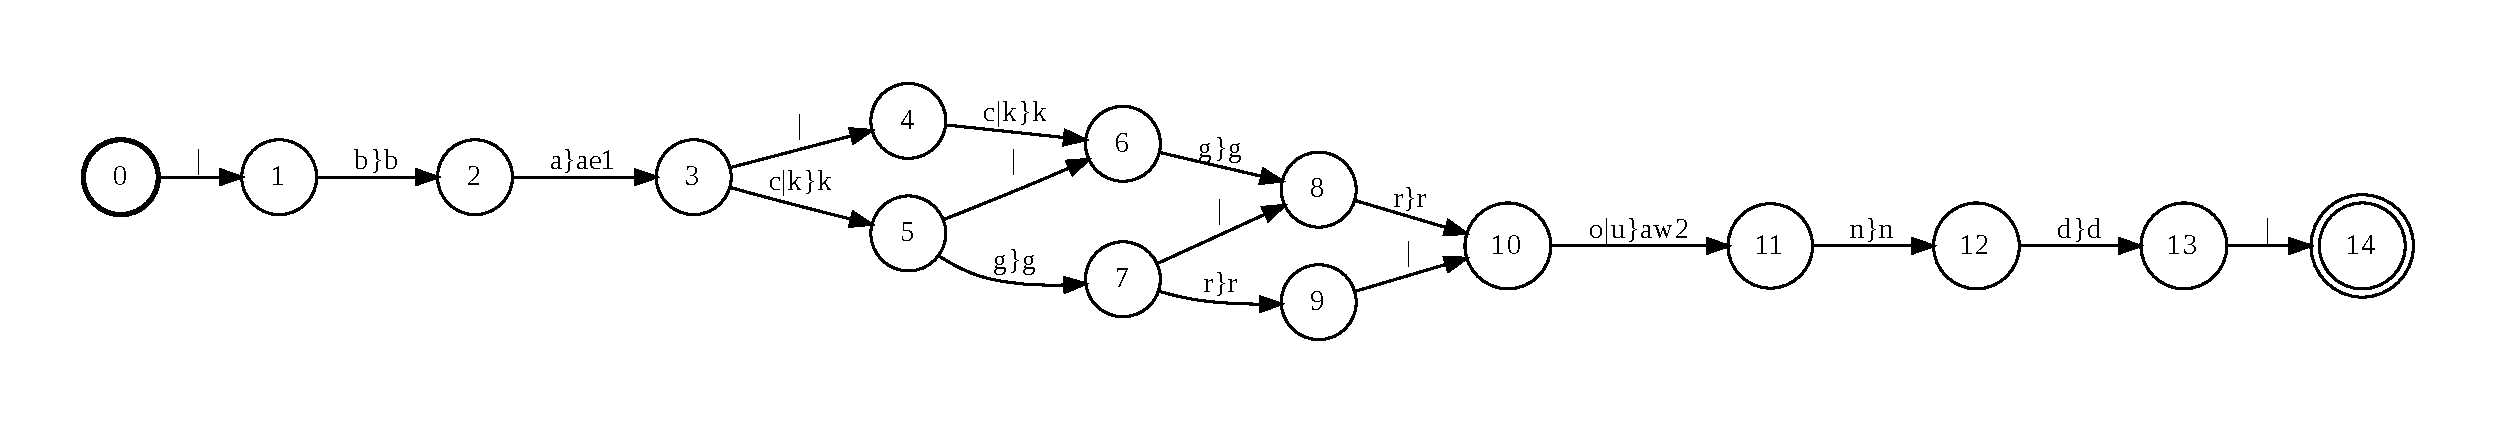
\includegraphics[width=320px]{fsa.pdf}
\end{figure}

\subsection{Training}
\label{ssect:train}

To get an idea of the comparative performance, two systems are needed: one using syllables, the other using phonemes. Kaldi~\citep{povey_kaldi_2011} contains a recipe for TIMIT; it is only set up for making a purely phoneme-based system, but the data preparation parts are still useful.

The phoneme-based system will use the TIMIT data as provided; the syllable-based system would need additional processing to extract the graphone-based syllables, using the model above, which would then be used as a basis for merging the timestamps of the phonetic transcripts, to create syllable transcripts. Once this data has been processed, the training procedure is the same as for the phoneme-based system, albeit using a differently segmented lexicon and language model.

\subsection{Evaluation}
\label{ssect:eval}

The motivation behind this experiment is to improve the performance of a speech recognition system; because of this, evaluation based on speech recognition is more informative than anything task-specific.

ASR systems are typically evaluated using Word Error Rate (WER) of the system's output, compared to a reference transcription. WER is formulated like so:

\[ \mathit{WER} = \frac{S+D+I}{N} = \frac{S+D+I}{S+D+C} \]

where $S$ is the number of substitutions, $D$ is the number of deletions, $I$ is the number of insertions, and $N$ is the total number of words in the reference transcription. 

Phone-based systems and character-based systems are often additionally evaluated using Phone Error Rate (PER) and Character Error Rate (CER), respectively. These can be useful in analysing the errors made by the system.

To perform a similar evaluation, the same formula can be used for ``Syllable Error Rate'', using syllables as input, though this would require re-segmenting the transcriptions of the test portion of the TIMIT corpus, as well as the training portion.

\section{Discussion}
\label{sect:discussion}

\subsection{Potential issues}
\label{ssect:issues}

The first potential issue is that, because the segmentation scheme has no explicit attempt to enforce restrictions on segment sequences, it could lead to unnatural segmentations. This could be addressed by adding an explicit mechanism for preventing such segmentations.

The next issue is the choice of corpus--TIMIT is quite small, and it's possible that the potential benefit of a larger basic unit would not be apparent without a sufficiently large training corpus.

Related to the above, another issue is the number of symbols: the TIMIT dictionary contains 6228 words; the simple syllabification method mentioned in subsection \ref{ssect:graphones} produced 6540 unique syllables, and of those, many contained two vowels: a more thorough segmentation system would produce more.

%An issue with my approach to the task is in how little attention I paid to the acoustic syllables. There are a number of methods for determining the locations of vowels in audio, but I came across the paper by \citet{dong_cif_2020} early on, which had a much better version of my idea, and I never quite came back to it.

%Also, the statistical syllabifier still doesn't exist; I've been trying to use the OpenFST ngram and baumwelch tools, which are as under-documented as the tools with OpenFST itself, and I'm starting to think that encoding a sentence FST doesn't work the way I want. The alternative approach is to recursively generate each possible path and weight them individually, so at least there's still scope for that to work.

\subsection{The premise}
\label{ssect:premise}

\subsubsection{Do syllables have a role as a unit for speech recognition?}

Although English is not unique in its difficulty regarding sentence boundaries (for example, \citet{goslin_comparing_2007} found that French presented similar difficulties), there are many languages for which the syllable is more central, and more clearly defined. Chinese is clearly one, as demonstrated by \citet{dong_cif_2020}.

An alternative unit might be a syllabic version of the phonetically-constrained morphological affixes presented by \citet{huckvale_using_2002}. \citet{tachbelie_morpheme-based_2010} mention that shorter morphological units are more confusable, but a syllable may be enough context to avoid that problem.

\subsubsection{The role of phonemes}

Although phoneme-based speech recognition is no longer to the fore of research, for practical speech recognition, it's likely that phonemes will continue to be useful. Languages do not exist in isolation: as I write this, Spain and Italy are playing in the semi-final of the Euros. Most, if not all, of these players will appear in at least the sporting news; few, if any, will be represented in a speech corpus.

Aside from general-purpose speech recognition, there are several other applications for speech recognition: for example, Computer-Assisted Pronunciation Training is a natural fit for phoneme-based speech recognition, because we want the learner to receive feedback when they use the wrong sound. It may be possible to simulate this using letters or words, but phonemes are the most obvious choice for that specific use case.

The joint word-letter learning of \citet{li_acoustic--word_2017} could be applied to joint phoneme-word or phoneme-syllable learning; \citet{zeyer_ctc_2017} found that CTC is a special case of Hidden Markov Models, while \citet{hannun_differentiable_2020} reformulated Weighted Finite-State Transducers to be differentiable, opening up possibilities of combining older methods with new; \citet{baevski_unsupervised_2021} use a mixture of old and new speech recognition systems for unsupervised learning.

\section{Conclusion}

In this report, I attempted to design an experiment to compare the syllable as a unit of speech with the phoneme. Lacking data specifically designed for the task, my primary focus was on using data that could be adapted to the task, and developing a means of adapting it, so that the comparison could be done in as conventional a way as possible.

%Once the alignment model $\hat{\Gamma}$ is estimated, we can use it to construct a so-called \textit{pair language model} (Novak et al. 2012, 2016). This is much like a classic language model but the actual symbols represent pairs in ${I} \times {O}$; unlike $\hat{\Gamma}$, it is a joint model. To construct such a model:
%1.  Compute the best $i, o$ alignments by decoding with $\hat{\Gamma}$.
%2.  Rewrite the FSTs in the decoded alignments FAR as acceptors over a pair symbol vocabulary ${I} \times {O}$.
%3.  Compute a higher-order language model (e.g., using the NGram tools), with standard smoothing and shrinking options, producing a weighted finite-state acceptor.
%4.  Convert the weighted finite-state acceptor to a finite-state transducer by rewriting the ``acceptor'' ${I} \times {O}$ arcs with the corresponding ``transducer'' ${I} : {O}$ arcs.
%Then the pair language model can be applied using composition and decoded using the Viterbi algorithm.

\bibliography{main}
%\bibliographystyle{apa}
%\nocite*{}

\end{document}